\subsection{Ablations and controlled negative controls}
\label{sec:pricing}

Of the three interfaces in Section~\ref{sec:interface}, only reservation-table-aware dispatching has a net gain under an equal wall-clock budget.
On the $\MatrixCells$-instance data of Section~\ref{sec:whichcongestion}, turning off yield-record feedback is \GainCertMatrix{} (significant on $1$ instance) and turning off staggering is \GainStaggerMatrix{} (significant on $2$).
Neither ablation worsens makespan, so the evaluations spent on these operators are better used by the population cycle.
This earlier batch may be cited for these two ablations---their cost does not depend on the speed-ups---but not for dispatching.
A $\theta$ scan on two $8\times4\times4$ instances (not Families A/B/C), collected before the speed-ups, is consistent with the observation of Section~\ref{sec:interface} that the surcharge adds no new information: under equal wall-clock every $\theta$ worsens makespan, flat over a ten-fold range; under equal evaluations the same comparison cannot be distinguished from zero.
Priced routing completes about one fifth as many evaluations, so the measured loss comes mainly from the multi-label search overhead of Lemma~\ref{lem:label}, so $\theta$ is not a useful parameter.

\label{sec:whycost}
The yield-record neighbourhood is small and directed (Section~\ref{sec:ls}), yet fewer than one in fifty neighbours improve makespan; three repairs of the operators were not significant under an equal number of evaluations.
Removing one corridor delay promotes another constraint, so the realized improvement is only a fraction of the wait removed (Figure~\ref{fig:case})---the same dilution that left dispatching in the noise at \CostMultBefore{} and significant after the multiple fell to \CostMultAfter{}.
The default therefore keeps dispatching and does not use the yield record to generate the neighbourhood.


\subsection{The cost law and the effect of the speed-ups}
\label{sec:costlaw}

The same dispatching rule is indistinguishable from noise before the speed-ups and significantly positive after them, so the speed-ups themselves are measured here.
Figure~\ref{fig:protocol} locks cost per evaluation and evaluations completed onto a shared wall-clock hyperbola.
The cheaper configuration completes more evaluations; the open loop uses less than two tenths of the wall-clock to complete the most.
Before the speed-ups, reservation-table-aware dispatching is \GainProbeSameGen{} ($p\PProbeSameGen$) at equal generation count and \GainProbeSameClock{} ($p\PProbeSameClock$) at equal wall-clock---almost zero.
Equal generation count asks whether the extra routing step improved that generation's ranking; equal wall-clock asks whether makespan fell in the same stretch of time.
Both questions are well posed, but they must not be conflated.

\begin{figure}[t]
\centering
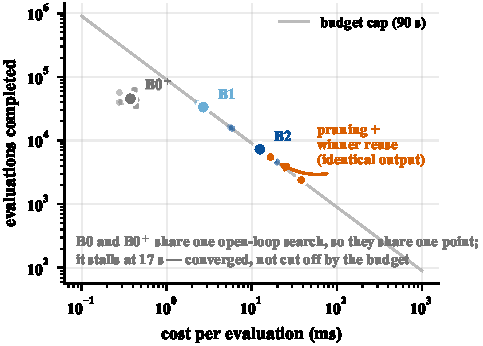
\includegraphics[width=0.7\columnwidth]{fig/fig_protocol.pdf}
\Description{A log-log scatter of cost per evaluation against evaluations
completed. A grey hyperbola marks the 90-second budget cap. The two closed-loop
configurations sit on it, while the open-loop configuration sits well below it
because it stalls after about seventeen seconds. Orange markers are the
pruning ablation off and on; a callout marks the on setting.}
\caption{Equal wall-clock time locks cost per evaluation and evaluations completed onto a hyperbola; the grey line is the shared $90$-second cap.
Closed-loop runs sit on the line; the open loop sits below it (early stop after $\sim$17\,s, Section~\ref{sec:protocol}).
B0 and B0$^+$ share a point.
Pale points are per-instance measurements on three instances; filled markers are their geometric mean, which preserves cost $\times$ count on a log axis.
Orange markers are pruning and winner-path reuse off and on (callout at the on setting): Proposition~\ref{prop:speedup_equiv} guarantees that the output does not change.}
\label{fig:protocol}
%% From fig/fig_protocol.py; ladder_cost.csv and prune_ablation.csv.
%% If the latter is missing the script omits the orange markers.
%% fig:protocols (two-convention bars) dropped; the pair
%% \GainProbeSameGen / \GainProbeSameClock is reported in the text.
\end{figure}

Reservation-table-aware dispatching raises the routing calls per transport task from $2$ to at most $2N_A$, so cost grows linearly with fleet size.
The pruning bound is tighter when contention is weaker; the larger the fleet and the stronger the contention, the smaller the cut.
The self-check of Section~\ref{sec:speedup} gives this direction: of six instances the highest cut is on the least congested one (\RouteCallCutHi{}) and the lowest on the largest fleet (\RouteCallCutLo{}).
The two trends \emph{predict} that when the fleet is large enough and contention strong enough, trial-query cost will offset the gain.
On the four $N_A/N_M$ levels of Section~\ref{sec:whichcongestion} the sign alternates and none is significant, so the upper bound is not confirmed.
The cost law itself (cost linear in $N_A$, pruning effect falling with $N_A$) is measured; the upper bound deduced from it is not.

The speed-ups and the dispatching rule were introduced one after the other, so a control that moves only the speed-ups is run: same instances, seeds, and budget.
Proposition~\ref{prop:speedup_equiv} guarantees that the two optimizations do not change the output.
On each of six instances six random chromosomes give makespans and dispatch sequences \emph{identical bit for bit} ($36$ groups, no exception); routing calls fall by \RouteCallCut{}.
Turning the optimizations off only makes one evaluation slower, so the equal-wall-clock difference comes only from saved compute.
Table~\ref{tab:prune}: off$\to$on reduces makespan by a further \GainPrune{} (\WinPrune{} wins / \LosePrune{} losses, $p\PPrune$); evaluations inside the same budget are \EvalRatioPrune{} times, and a single evaluation is sped up by \SpeedupProbe{}.
The same rule is \GainProbePre{} on the pre-speed-up matrix batch (significant on $0$ of the $\MatrixCells$ instances) and significantly positive on the post-speed-up ladder; the step in between did not change any selection.

\begin{table}[t]
\caption{Pruning and winner-path reuse off versus on (bold header: the setting used here).
Output is bit-identical, so the difference is saved compute.
Same instances, seeds, and wall-clock; $n=60$ pairs, two-sided Wilcoxon ($^{***}p<0.001$).
Ratio columns take the off setting as denominator, in opposite directions.}
\label{tab:prune}
\small
%% Regenerated from prune_ablation.csv by gen_tables_ladder.py.
%% 由 tab/gen_tables_ladder.py 生成,请勿手工编辑
%% 数据源:clbs/output/baseline_ladder.csv 等,见脚本首部
\begin{tabular}{@{}lrrrrrr@{}}
\toprule
& & \multicolumn{2}{c}{$C_{\max}$ (time units)} & & Eval.\ count ratio & Speedup per eval. \\
\cmidrule(lr){3-4}
Instance & Contention & Off & \textbf{On} & $\Delta C_{\max}$ & (on/off) & (off/on) \\
\midrule
A funnel & 31.9\% & 44.80 & 42.10 & $-6.03\%$ & 2.21$\times$ & 2.23$\times$ \\
A high & 30.9\% & 41.60 & 37.70 & $-9.37\%$ & 2.40$\times$ & 2.41$\times$ \\
A low & 11.8\% & 60.50 & 57.00 & $-5.79\%$ & 2.79$\times$ & 2.81$\times$ \\
B NA/NM 0.5 & 15.8\% & 66.70 & 65.10 & $-2.40\%$ & 2.11$\times$ & 2.11$\times$ \\
B NA/NM 1.0 & 30.2\% & 51.90 & 48.90 & $-5.78\%$ & 2.31$\times$ & 2.31$\times$ \\
B NA/NM 2.0 & 32.4\% & 44.50 & 42.20 & $-5.17\%$ & 1.98$\times$ & 2.01$\times$ \\
\midrule
\emph{Pooled} (60 pairs) & --- & --- & --- & $-5.60\%^{***}$ & \multicolumn{2}{r}{50/0/10,\ $<10^{-4}$} \\
\midrule
\multicolumn{7}{@{}l@{}}{\footnotesize HL pseudomedian and $95\%$ CI:$-4.72$ $[-6.34,-3.55]$\,\%} \\
\bottomrule
\end{tabular}

\end{table}

\subsection{Case study: Gantt chart and critical chain on the funnel instance}
\label{sec:casestudy}

Figure~\ref{fig:case} places B0 and B2 on one funnel instance: arms and vehicles share a time axis, and the critical chain is coloured by Table~\ref{tab:attrib}.
In the open-loop solution, yielding wait appears near the station and concentrates on a few vehicles.
The closed-loop solution cuts those waits and assigns several operations to an arm that is not the fastest---assignments of the \eqref{eq:reassign} kind---and, as a consequence rather than a third mechanism, balances vehicle idle and busy time more evenly.
On B0's chain \texttt{corridor} occupies a substantial share; on B2 those links largely disappear, and \texttt{machine} and \texttt{upstream} come to the top.
That is the dilution of Section~\ref{sec:whycost}: remove one corridor delay, and another constraint becomes tight.

\begin{figure*}[t]
\centering
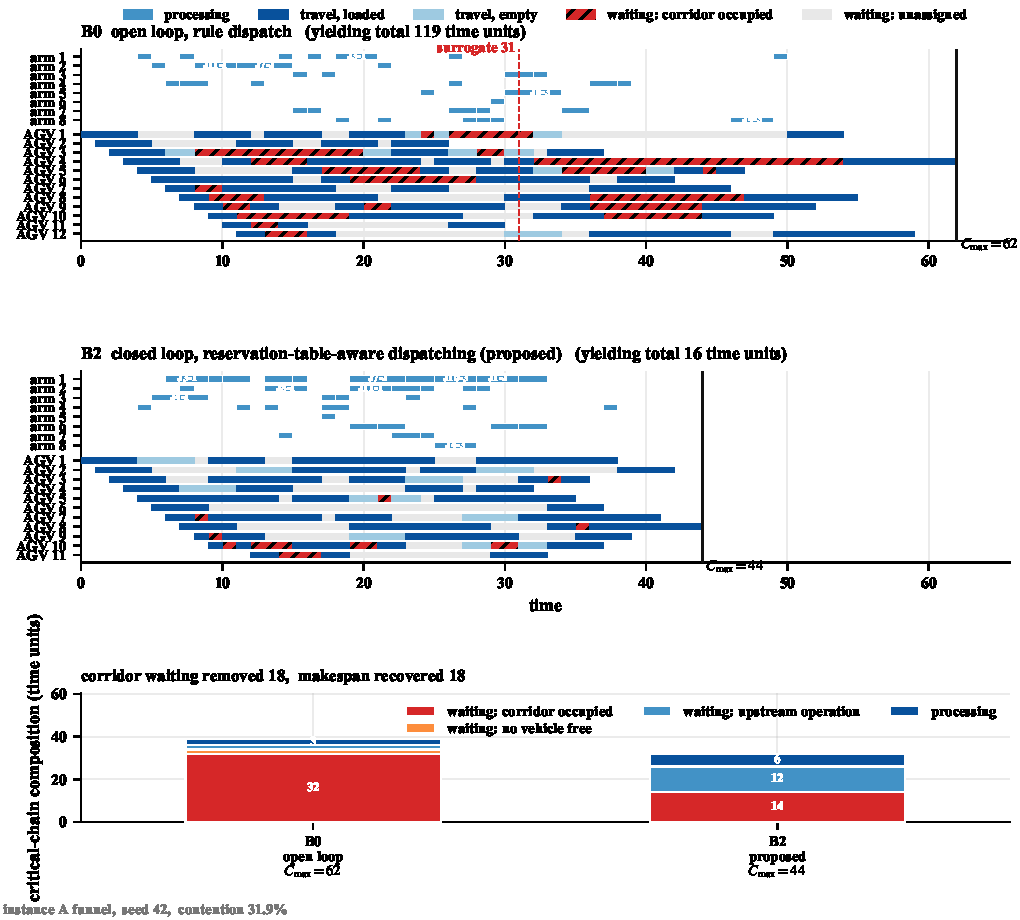
\includegraphics[width=\textwidth]{fig/fig_case.pdf}
\Description{Two Gantt charts of the open-loop and closed-loop solutions on one
funnel instance, with arms and vehicles on a shared time axis, followed by
stacked bars that decompose each critical chain by attribution label.}
\caption{B0 and B2 on one funnel instance (existence reading, not a statistical claim).
Top: arms and vehicles on a shared time axis; a gap inside one transport is yielding wait, a gap between tasks is idle time.
Bottom: critical-chain composition by Table~\ref{tab:attrib}; corridor wait removed versus makespan recovered is the dilution of Section~\ref{sec:whycost}.}
\label{fig:case}
%% From fig/fig_case.py and case_study/*.json (ladder_diag.py --case-study).
%% Merges the former fig_case_gantt / fig_case_chain pair.
\end{figure*}

\subsection{Degenerate comparison on public benchmarks}
\label{sec:external}

The preceding sections compared configurations of the same codebase; they cannot calibrate the absolute level of the implementation.
After \eqref{eq:excl} is removed the model degenerates to standard FJSP\_PT, the \emph{same mathematical problem} as the public benchmarks; $\delta_{\mathrm{ret}}=0$ aligns the makespan definition (Table~\ref{tab:notation}).
Neither mechanism enters; what is tested is the \emph{upper-level search}.

The \PubNInst{} instances compiled by Homayouni and Fontes~\cite{homayouni2021production} (originating in Fattahi et al.~\cite{fattahi2007mathematical}) are taken with two vehicles as in the literature~\cite{lim2023twophase} and no return of finished goods.
Travel times are used as published: \PubNLayoutBad{} of the matrices are not a shortest-path closure, and a synthesis would change the instance.
\PubNOpt{} instances have a MILP-proven optimum~\cite{homayouni2021production}; the remaining $4$ take the published best-known~\cite{lim2023twophase}.

Table~\ref{tab:external} is \PubNInst{} instances $\times$ \NSeeds{} seeds.
All $200$ runs pass the validator and the composite lower bound; on the \PubNOpt{} proven-optimum instances no run falls below that value.
On $\PubNMatch{}/\PubNInst{}$ instances the best solution is identical bit for bit to the reference, including all $10$ small instances; the mean gap is \PubGapMean{} (median \PubGapMed{}).
The four largest instances have mean \PubGapBig{}, worst \PubGapMax{}; none of the $16$ instances with at most $24$ operations exceeds $5.45\%$.

\begin{table}[t]
\caption{Degenerate comparison on public benchmarks (exclusivity removed).
\textsc{opt}: MILP-proven optimum; \textsc{bk}: published best-known; gap from the best of \NSeeds{} seeds.
An asterisk marks a bitwise-identical best solution.}
\label{tab:external}
\centering
\small
%% 由 tab/gen_tables_ladder.py 生成,请勿手工编辑
%% 数据源:clbs/experiments_database/gap_ideal.csv;工序数取自 clbs/database/json/hf/*.json
\begin{tabular}{lrrrrrr}
\toprule
& & & \multicolumn{3}{c}{$C_{\max}$ (time units)} & \\
\cmidrule(lr){4-6}
Instance & Ops & Ref. & \multicolumn{1}{c}{Value} & Best & Mean & Gap \\
\midrule
SFJST01 & 4 & \textsc{opt} & 70 & 70\rlap{$^*$} & 70.0 & 0.00\% \\
SFJST02 & 4 & \textsc{opt} & 111 & 111\rlap{$^*$} & 111.0 & 0.00\% \\
SFJST03 & 6 & \textsc{opt} & 223 & 223\rlap{$^*$} & 223.0 & 0.00\% \\
SFJST04 & 6 & \textsc{opt} & 359 & 359\rlap{$^*$} & 359.0 & 0.00\% \\
SFJST05 & 6 & \textsc{opt} & 123 & 123\rlap{$^*$} & 123.0 & 0.00\% \\
SFJST06 & 9 & \textsc{opt} & 324 & 324\rlap{$^*$} & 324.0 & 0.00\% \\
SFJST07 & 9 & \textsc{opt} & 409 & 409\rlap{$^*$} & 409.0 & 0.00\% \\
SFJST08 & 9 & \textsc{opt} & 269 & 269\rlap{$^*$} & 269.5 & 0.00\% \\
SFJST09 & 9 & \textsc{opt} & 220 & 220\rlap{$^*$} & 222.0 & 0.00\% \\
SFJST10 & 12 & \textsc{opt} & 531 & 531\rlap{$^*$} & 531.0 & 0.00\% \\
MFJST01 & 15 & \textsc{opt} & 485 & 485\rlap{$^*$} & 485.0 & 0.00\% \\
MFJST02 & 15 & \textsc{opt} & 463 & 476 & 483.4 & 2.81\% \\
MFJST03 & 18 & \textsc{opt} & 482 & 482\rlap{$^*$} & 504.7 & 0.00\% \\
MFJST04 & 21 & \textsc{opt} & 576 & 586 & 623.0 & 1.74\% \\
MFJST05 & 21 & \textsc{opt} & 532 & 561 & 592.8 & 5.45\% \\
MFJST06 & 24 & \textsc{opt} & 652 & 677 & 728.3 & 3.83\% \\
MFJST07 & 32 & \textsc{bk} & 898 & 965 & 1023.3 & 7.46\% \\
MFJST08 & 36 & \textsc{bk} & 900 & 970 & 1027.0 & 7.78\% \\
MFJST09 & 44 & \textsc{bk} & 1098 & 1226 & 1279.2 & 11.66\% \\
MFJST10 & 48 & \textsc{bk} & 1230 & 1389 & 1473.0 & 12.93\% \\
\bottomrule
\end{tabular}

\end{table}
%% tab_external() from gap_ideal.csv; the Ops column is counted from
%% hf/*.json (len(proc_time)), not typed.  The same function prints the \Pub*
%% macros.  Edit the CSV, then re-run the script.

Raising the budget on the $10$ \textsc{mfjst} instances (\PubBudgetRatio{} times the wall-clock, generation cap five times) cuts their mean gap from \PubGapLoBudget{} to \PubGapHiBudget{} ($\PubBudgetGainPP$ percentage points); none of the $300$ runs hits the generation cap---a capability boundary, not a short budget (item~(3) of Section~\ref{sec:future_work}).
On the \PubNOpt{} proven-optimum instances the composite lower bound lies a median \PubLBSlack{} below the optimum and \PubLBTotal{} below this paper's best; the search shortfall is a median $\PubLBResidMed$ percentage points and at most $\PubLBResidMax$, so almost all of the gap is slack in the bound.
The self-generated instances cannot inherit this proportion: their bound contains no contention, so \LBGapMed{} \emph{must not} be read as a search gap (limitation~(3) of Section~\ref{sec:limitations}).



\section{Conclusion}

Flexible assignment and conflict-free AGV routing must be decided jointly: travel time is produced by routing, and when the corridor to a fast arm is congested, a slower, better-connected arm may be the better assignment.
Existing methods schedule on a constant matrix or freeze the assignment first, so yielding wait does not enter the evaluation of candidates.
Our bilevel framework connects the two levels by an evaluation path and a decision path and measures them separately under the same wall-clock budget; because a conflict-free evaluation is more than an order of magnitude more expensive than a matrix lookup, it also includes output-preserving speed-ups.

\subsection{Findings and contributions}
\label{sec:contributions}

The four contributions of Section~\ref{sec:Chapter_I} are restated with their supporting numbers.
\begin{enumerate}[leftmargin=*,topsep=2pt,itemsep=2pt]
\item \textbf{Instances.} On top of the problem setting of~\cite{vanos2026exact}, instance families with controllable contention intensity characterize how high contention must be before counting yielding wait in the schedule yields a gain (Section~\ref{sec:whichcongestion}).
\item \textbf{Evaluation.} Routing-in-the-loop evaluation reduces makespan by $\GainLoopRule$ under rule-based dispatching ($p\PLoopRule$) and by $\GainLoopProbe$ under reservation-table-aware dispatching ($p\PLoopProbe$).
Proposition~\ref{prop:decodable} and Lemma~\ref{lem:label} guarantee that every chromosome is decodable and that the evaluation matches the conflict model of Section~\ref{sec:Chapter_III}.
\item \textbf{Dispatching.} Within the closed loop, trial-querying both legs reduces makespan by a further $\GainProbeLoop$ ($p\PProbeLoop$).
Admissible lower-bound pruning and winner-path reuse change neither the selected vehicle nor the timetable (Proposition~\ref{prop:speedup_equiv}), cut router calls by \RouteCallCut{}, and lower the cost multiple from \CostMultBefore{} to \CostMultAfter{}.
\item \textbf{Evidence.} The two paths differ in magnitude, are near-additive, and are not substitutes.
The closed loop remains significant after Holm correction on \CellsSigLoopAdj{} of the $\NCases$ instances; dispatching is significant only when pooled ($95\%$ interval \CIProbeLoop{}) and on no instance individually.
The end-to-end $\GainEndToEnd$ is close to the prediction under independent composition, $\GainIndepProduct$ (no positive interaction detected); open-loop dispatching ($\GainProbeOpen$) cannot replace the closed loop.
A surcharge on occupied corridor--time slots, and reassignment or staggering from the yield record, do not further reduce makespan under the same budget.
\end{enumerate}

\subsection{Limitations and future work}
\label{sec:limitations}
\label{sec:future_work}

\textbf{(1) Instance families.}
The main experiment fixes size and varies only structure (Section~\ref{sec:features}), so we draw no conclusion about how the mechanisms vary with size.
$H$ is fixed at $0.3$; ``the gain does not rise with $H$'' comes from the smaller independent batch of Section~\ref{sec:whichcongestion} and holds only at that size.
The layout family is spliced from two topologies: the three dumbbells change only capacity, while the two grids change topology and distance together (\LegDumbbell{} versus \LegGrid{}, Section~\ref{sec:instances}).
Contention intensity is a one-dimensional measure that does not separate the wait reassignment can bypass, so only the differences among the three dumbbells can be attributed to capacity alone.
Self-generated instances are used because no usable public benchmark exists: common FJSP\_PT benchmarks publish constant matrices, \PubNLayoutAsym{}/\PubNLayout{} of the examined matrices are asymmetric and \PubNLayoutBad{} are not a shortest-path closure (Section~\ref{sec:instances}), and works with an explicit road network use different reservation units (Section~\ref{sec:fjsppt}).
Future work should remeasure on a larger corridor network and treat ``whether congestion can be bypassed by reassignment'' and ``whether the critical chain has a single dominant bottleneck'' as separate factors; $\varphi$ failed to separate the corresponding layout classes.

\textbf{(2) Dispatching is positive on average, but its per-instance stability is not yet determined.}
$\NSeeds$ seeds suffice for the closed loop ($\CellsSigLoopAdj/\NCases$ after Holm).
The effect of reservation-table-aware dispatching is a few percentage points, of the same order as the seed-to-seed dispersion: $\CellsSigProbe/\NCases$ instances are significant before correction and $\CellsSigProbeAdj/\NCases$ after, so the gain is confirmed as positive only on the $\NPairs$ pooled pairs ($95\%$ interval \CIProbeLoop{}).
About an order of magnitude more seeds, and denser $N_A/N_M$ levels, would be needed to determine the class of instances on which it is stable and to test the cost-law upper bound of Section~\ref{sec:costlaw}.

\textbf{(3) The distance of solutions from the optimum under corridor contention is unknown.}
The configurations share one code base, so the strength of the upper-level search does not affect the differences among levels.
Section~\ref{sec:external} is bitwise identical to the literature on $\PubNMatch{}/\PubNInst{}$ instances, and all $10$ small instances reach a proven optimum.
The four largest average \PubGapBig{}, and \PubBudgetRatio{} times the compute improves this by only $\PubBudgetGainPP$ percentage points, so the gap reflects a capability limit rather than an insufficient budget.
On the \PubNOpt{} proven-optimum instances the search solution is at most $\PubLBResidMax$ percentage points from the optimum, and the bound gap comes almost entirely from slack in the bound.
On the self-generated instances the bound contains no contention, so its median gap \LBGapMed{} cannot be read as a search gap; a secondary effect of a few percentage points such as \GainProbeLoop{} may be of the same order as the unknown distance to the optimum.
Exact solutions by logic-based Benders decomposition~\cite{vanos2026exact} on small contended instances would separate bound slack from search shortfall.

\textbf{(4) The surcharge and yield-record-guided local search must be remeasured if their own cost is reduced.}
Both were assessed in the same code base under the same wall-clock budget, so what was measured is the trade-off between cost per evaluation and number of evaluations.
Speeding up all configurations by the same factor leaves that trade-off and the sign unchanged; only reducing the cost of one interface separately could change the sign, as the dispatching speed-ups of Section~\ref{sec:speedup} illustrate.
Re-solving only the perturbed suffix of a chromosome would allow that local search to be remeasured under the same wall-clock budget.

\textbf{(5) Failures and online arrivals are out of scope.}
Assumption A7 excludes robotic-arm and vehicle failures and dynamic arrivals from the model.
The reported results hold for a static horizon; with failures or online arrivals, the value of a mechanism also includes how fast it repairs a schedule~\cite{gui2023dynamic,xiong2024dynamic,dauzereperes2024fjsp}.


%\section*{Acknowledgments}
%This work was supported partly by Key Laboratory of Computer Network and Information Integration (Southeast University) of Ministry of Education of China under Grants NO. 93K-9 and Jiangsu Provincial Key Laboratory of Network and Information Security under Grants No.BM2003201.

%%
%% The next two lines define the bibliography style to be used, and
%% the bibliography file.
\bibliographystyle{ACM-Reference-Format}
\bibliography{reference-base}


%% No appendix.  An empty \appendix leaves a blank TOC/header entry in acmart.

\end{document}
\endinput
%%

